\documentclass[letterpaper,10pt]{article}

\usepackage{fullpage}

\usepackage{amsmath}
\usepackage{amssymb}
\usepackage{amsthm}
\usepackage{tikz}

\title{Drawing A Graph With Tikz}
\author{Craig Kelly}

\begin{document}

% Force pdflatex to properly use letter as page size (instead
% of defaulting to A4)
\special{papersize=8.5in,11in}
\setlength{\pdfpageheight}{\paperheight}
\setlength{\pdfpagewidth}{\paperwidth}

\setlength{\parindent}{0pt}
\setlength{\parskip}{6pt}

\maketitle

\section*{Here's a simple graph}

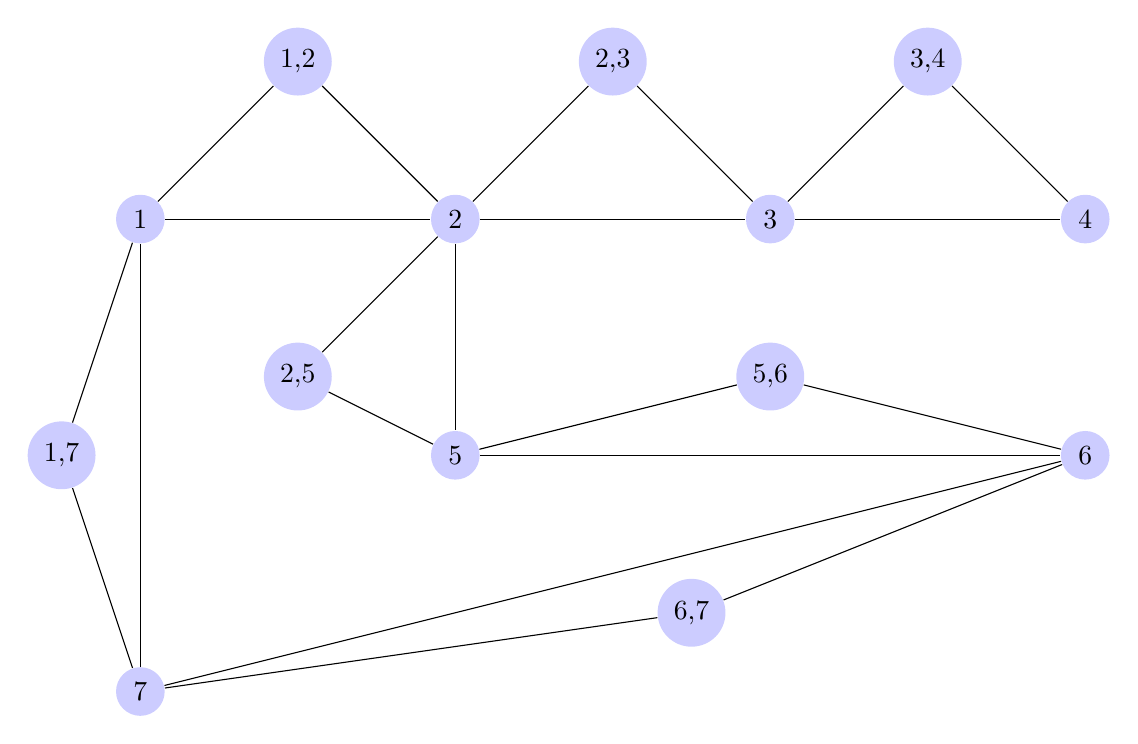
\begin{tikzpicture}
    [scale=1.0,auto=left,every node/.style={circle,fill=blue!20}]
    \node (n1) at (1,7)  {1};
    \node (n2) at (5,7)  {2};
    \node (n3) at (9,7)  {3};
    \node (n4) at (13,7) {4};
    \node (n5) at (5,4)  {5};
    \node (n6) at (13,4) {6};
    \node (n7) at (1,1)  {7};
    \node (n12) at (3,9)  {1,2};
    \node (n23) at (7,9)  {2,3};
    \node (n34) at (11,9) {3,4};
    \node (n17) at (0,4)  {1,7};
    \node (n25) at (3,5)  {2,5};
    \node (n56) at (9,5)  {5,6};
    \node (n67) at (8,2)  {6,7};

    \foreach \from/\to in {n1/n2,n2/n3,n3/n4,n1/n7,n2/n5,n5/n6,n6/n7}
    \draw (\from) -- (\to);
    
    \foreach \from/\to in {n1/n12,n2/n12} \draw (\from) -- (\to);
    \foreach \from/\to in {n2/n23,n3/n23} \draw (\from) -- (\to);
    \foreach \from/\to in {n3/n34,n4/n34} \draw (\from) -- (\to);
    \foreach \from/\to in {n1/n17,n7/n17} \draw (\from) -- (\to);
    \foreach \from/\to in {n2/n25,n5/n25} \draw (\from) -- (\to);
    \foreach \from/\to in {n5/n56,n6/n56} \draw (\from) -- (\to);
    \foreach \from/\to in {n6/n67,n7/n67} \draw (\from) -- (\to);
\end{tikzpicture}

\end{document}
